% nt-03-freud.tex

\documentclass[xcolor=dvipsnames]{beamer}
\usepackage{teachbeamer}

\title{Nietzsche and Freud}
\subtitle{{\CourseNumber}, {\CourseInst}}

\author{\CourseName}

\date{May 29, 2018}

\begin{document}

\begin{frame}
  \titlepage
\end{frame}

% \begin{frame}
%   \frametitle{iClicker Question}
% Choose from the following options. This item will be graded.
% \begin{block}{iClicker Question}
% [2482] Which one of these infantile activities does Freud address at length?
% \end{block}
% \begin{description}
% \item[A\hspace{.2in}$\blacktriangleright$] Bedwetting
% \item[B\hspace{.2in}$\blacktriangleright$] Sleepwalking
% \item[C\hspace{.2in}$\blacktriangleright$] Thumbsucking
% \item[D\hspace{.2in}$\blacktriangleright$] Pottytraining
% \end{description}
% \end{frame}

% \begin{frame}
%   \frametitle{iClicker Question}
% Choose from the following options. This item will be graded.
% \begin{block}{iClicker Question}
% [1440] What are Freud's ``psychical dams''?
% \end{block}
% \begin{description}
% \item[A\hspace{.2in}$\blacktriangleright$] ego, id, super-ego
% \item[B\hspace{.2in}$\blacktriangleright$] shame, disgust, and morality
% \item[C\hspace{.2in}$\blacktriangleright$] dreams, jokes, Freudian slips
% \item[D\hspace{.2in}$\blacktriangleright$] sublimation, elimination, projection
% \end{description}
% \end{frame}

% \begin{frame}
%   \frametitle{iClicker Question}
% Choose from the following options. This item will be graded.
% \begin{block}{iClicker Question}
% [3484] In Mattia Riccardi's paper, Nietzsche is interpreted to claim
% that a Newton of psychology would find causal, not teleological,
% explanations for behaviour and actions. What, according to Nietzsche,
% are the components of these causal explanations?
% \end{block}
% \begin{description}
% \item[A\hspace{.2in}$\blacktriangleright$] drives
% \item[B\hspace{.2in}$\blacktriangleright$] volitions
% \item[C\hspace{.2in}$\blacktriangleright$] goals
% \item[D\hspace{.2in}$\blacktriangleright$] commands
% \end{description}
% \end{frame}

% \begin{frame}
%   \frametitle{iClicker Question}
% Choose from the following options. This item will be graded.
% \begin{block}{iClicker Question}
% [2627] In philosophy, ``privacy'' is the term for access to your own
% mental states; ``mindreading'' is the term for access to other
% people's mental states. Which of the following is closest to
% Nietzsche's view, according to Mattia Riccardi's paper?
% \end{block}
% \begin{description}
% \item[A\hspace{.2in}$\blacktriangleright$] privacy is transparent, mindreading is obscured
% \item[B\hspace{.2in}$\blacktriangleright$] privacy gives us privileged access to our own mental states
% \item[C\hspace{.2in}$\blacktriangleright$] mindreading is possible only on the basis of privacy
% \item[D\hspace{.2in}$\blacktriangleright$] privacy is as obscured as mindreading
% \end{description}
% \end{frame}

\begin{frame}
  \frametitle{Psycho-Analysis} 
  Many of the things that Freud said were pre-empted by Nietzsche, for
  example the idea of the subconscious. Both Freud and Nietzsche were
  thinkers who were trying to understand what an honest intellectual
  response to the historical phenomenon of modernity could look like.
  Modernity is where
\begin{quote}
  {\ldots} the people have lost their ancient beliefs; the parson sits
  at home and unravels his vestments, one after another {\ldots}
  (Franz Kafka, A Country Doctor, 141)
\end{quote}
\end{frame}

\begin{frame}
  \frametitle{Markers of Modernity} 
  \begin{description}
  \item[epistemological crisis] ``I was in great perplexity'' (136)
  \item[the efficiency of aimlessness] ``you never know what you are
    going to find in your own house'' (137)
  \item[the twinning of pathology and sex] the boy's wound (141)
    Kafka's bisexuality? See Foucault's \emph{History of Sexuality}
  \item[lack of agency] first, the doctor cannot help because the boy
    is healthy; then he cannot help because the boy is past helping (141)
  \item[collapse of eschatology] ``it cannot be made good, not ever''
    (143)
  \end{description}
\end{frame}

\begin{frame}
  \frametitle{Ontogenesis vs. Phylogenesis} Another parallel between
  Nietzsche and Freud is that both were trying to do to psychology
  what Darwin did with respect to life: explain by revealing its
  history. The important difference for Freud is that he used
  \alert{ontogenesis} instead of \alert{phylogenesis} for his
  explanation (25). Here are some key concepts in psycho-analysis.
\end{frame}

\begin{frame}
  \frametitle{Key Concepts I} 
  \begin{description}
  \item[drives] irrational drives determine human behaviour; rational
    explanations are epiphenomenal (confabulation)
  \item[neurosis] conflict between the unconscious and the conscious
    creates repression
  \item[subconscious] the wall between the unconscious and the
    conscious is porous, but information which passes through is
    encrypted in symbols (dreams, myths, jokes, Freudian slips)
  \item[psycho-analysis] therapy is bringing-to-consciousness and
    transference (32)
  \end{description}
\end{frame}

\begin{frame}
  \frametitle{Key Concepts II} 
  \begin{description}
  \item[Oedipus Complex] early childhood amnesia obscures the Oedipus
    complex
  \item[Id Ego Superego] the rational identity is confronted with an
    animalic identity and with a repressive identity (double object
    selection, separated by latency, 37) (for ``id'' see the groom in
    ``A Country Doctor'' (137), for ``superego'' see the priest in ``The
    Trial'')
  \item[sex] the explanatory power of sex (16), although sexual desire
    ultimately must be sublimated (19, 26) (and, sometimes, a cigar is
    just a cigar, 40)
  \end{description}
\end{frame}

\begin{frame}
  \frametitle{Highlights of Infantile Sexuality} 
  \begin{itemize}
  \item primeval history and amnesia: ``infantile amnesia turns the
    childhood of each individual into something like a prehistoric
    past'' (37)
  \item the importance of latency
  \item sexual innocence and exaggerated sexual desire (16)
  \item notice how Freud struggles to define abnormality (19, see his
    dam analogy on page 26)
  \end{itemize}
\end{frame}

\begin{frame}
  \frametitle{Psychological Dams}
  It is a well-known trope in psychotherapy that the water will
  eventually find its way downhill, but it is in some sense left to
  the will to bar or encourage its flow. Freud identifies three
  psychological dams:
  \begin{itemize}
  \item disgust
  \item feelings of shame
  \item aesthetic and moral ideals
  \end{itemize}
\end{frame}

\begin{frame}
  \frametitle{Nietzsche and Freud}
  One way in which Freud stands in contrast to Nietzsche is the way in
  which Freud encourages development into a ``normal and enculturated
  individual'' (39). One of Freud's famous tools for this development
  is \alert{sublimation}: ``diversion of sexual driving forces from
  sexual aims and their direction to new ones'' (39). 
\end{frame}

\begin{frame}
  \frametitle{Freud on Gender}
  Both Freud and Nietzsche have their misogynist moments, but in quite
  different ways. 
  \begin{itemize}
  \item ``the preference for the hand already suggests the important
    contribution that the drive for mastery will later make toward
    masculine sexual activity'' (48)
  \item ``under ordinary conditions, she may remain normal sexually,
    but if led on by a skillful seducer, she will develop a taste for
    every sort of perversion'' (50)
  \end{itemize}
\end{frame}

\begin{frame}
  \frametitle{Newton of Psychology}
  The holy grail of psychology:
  \begin{itemize}
  \item identify the principal explanatory tokens of behaviour
  \item provide a causal rather than a teleological explanation of behaviour
  \end{itemize}
The phenomenology of an action is such that it appears to be caused
by a volitional state, by a willing. This is a primeval delusion.
\end{frame}

\begin{frame}
  \frametitle{Inner Opacity}
  Riccardi's \emph{Inner Opacity} view implies the following:
  \begin{itemize}
  \item it is false that we are directly aware of our mental states
  \item self-knowledge (privacy) is not privileged over
    other-knowledge (mind-reading)
  \end{itemize}
\end{frame}

\begin{frame}
  \frametitle{Inner Opacity}
  The following play a crucial role in the Inner Opacity view:
  \begin{description}
  \item[folk psychology] language and the phenomenology of conscious
    attitudes
  \item[consciousness] consciousness is a surface and sign world, a
    world of generalities, ``all becoming conscious involves a vast
    and thorough corruption, falsification, superficialization, and
    generalization'' (Gay Science, 354)
  \item[drives] homuncularist and dispositionalist interpretation
    (Riccardi's functionalist reading)
  \end{description}
\end{frame}

\begin{frame}
  \frametitle{Cognitive Science}
  Some views from cognitive science that are informative with respect
  to Nietzsche's view:
  \begin{description}
  \item[Alvin Goldman] mind-reading is primarily simulation
  \item[Alison Gopnik] mind-reading is primarily theory
  \item[Peter Carruthers] self-knowledge is primarily theory
  \end{description}
According to the IO view, ``the same set of cognitive capacities
enables both introspective self-knowledge and outward-directed
mind-reading'' (226). James Sully's ``obscure region of
self-consciousness'' (231).
\end{frame}

% \begin{frame}
%   \frametitle{iClicker Question}
% Choose from the following options. This item will be graded.
% \begin{block}{iClicker Question}
% [2255] According to John Richardson, what is the effect of
% consciousness and choosing in Nietzsche's psychological theory?
% \end{block}
% \begin{description}
% \item[A\hspace{.2in}$\blacktriangleright$] it is effective at turning us into rational choosers
% \item[B\hspace{.2in}$\blacktriangleright$] it is effective at turning us into herd animals
% % replace this item or give half mark
% \item[C\hspace{.2in}$\blacktriangleright$] it is ineffective (epiphenomenal)
% \item[D\hspace{.2in}$\blacktriangleright$] it is the effective feature of an aristocratic strong person (a master)
% \end{description}
% \end{frame}

% \begin{frame}
%   \frametitle{iClicker Question}
% Choose from the following options. This item will be graded.
% \begin{block}{iClicker Question}
% [6465] Richardson's account of freedom in Nietzsche is based on the following core result.
% \end{block}
% \begin{description}
% \item[A\hspace{.2in}$\blacktriangleright$] Nietzsche accepts and improves the traditional account of freedom in terms of agency and choice
% \item[B\hspace{.2in}$\blacktriangleright$] Nietzsche rejects a dynamic view of freedom and claims that it is metaphysically simple and unchanging
% \item[C\hspace{.2in}$\blacktriangleright$] Nietzsche rejects a traditional account of freedom and seeks to provide a new account
% \item[D\hspace{.2in}$\blacktriangleright$] Nietzsche rejects freedom under any description
% \end{description}
% \end{frame}

% \begin{frame}
%   \frametitle{iClicker Question}
% Choose from the following options. This item will be graded.
% \begin{block}{iClicker Question}
% [7397] Which of these characters occur in the \emph{Daybreak} Nietzsche reading?
% \end{block}
% \begin{description}
% \item[A\hspace{.2in}$\blacktriangleright$] Leibniz, Napoleon, Queen Victoria
% \item[B\hspace{.2in}$\blacktriangleright$] Pascal, Luther, St. Paul
% \item[C\hspace{.2in}$\blacktriangleright$] Mill, Freud, Hegel
% \item[D\hspace{.2in}$\blacktriangleright$] Kierkegaard, Schelling, Mozart
% \end{description}
% \end{frame}

% \begin{frame}
%   \frametitle{iClicker Question}
% Choose from the following options. This item will be graded.
% \begin{block}{iClicker Question}
% [3745] Which of these quotes is Nietzsche's?
% \end{block}
% \begin{description}
% % Freud
% \item[A\hspace{.2in}$\blacktriangleright$] A certain degree of neurosis is of inestimable value as a drive, especially to a psychologist.
% % Nietzsche
% \item[B\hspace{.2in}$\blacktriangleright$] Our intellect is only the blind instrument of another drive which is a rival of the drive whose vehemence is tormenting us
% % Lincoln
% \item[C\hspace{.2in}$\blacktriangleright$] I pass my life in preventing the storm from blowing down the tent, and I drive in the pegs as fast as they are pulled up.
% % ML King
% \item[D\hspace{.2in}$\blacktriangleright$] Darkness cannot drive out darkness; only light can do that. Hate cannot drive out hate; only love can do that.
% \end{description}
% \end{frame}

% \begin{frame}
%   \frametitle{iClicker Question}
% Choose from the following options. This item will be graded.
% \begin{block}{iClicker Question}
% [8323] According to Janaway's interpretation of Nietzsche, what brings about feelings of guilt?
% \end{block}
% \begin{description}
% % replace this item
% \item[A\hspace{.2in}$\blacktriangleright$] transgressing divine commands
% \item[B\hspace{.2in}$\blacktriangleright$] failing to follow Nietzsche's recommendation how to live a good life
% \item[C\hspace{.2in}$\blacktriangleright$] violating sexual taboos
% \item[D\hspace{.2in}$\blacktriangleright$] internalizing the drive to cruelty and expression of power
% \end{description}
% \end{frame}

% \begin{frame}
%   \frametitle{iClicker Question}
% Choose from the following options. This item will be graded.
% \begin{block}{iClicker Question}
% [3760] Which of these does Janaway seek to explain in his Nietzsche interpretation?
% \end{block}
% \begin{description}
% \item[A\hspace{.2in}$\blacktriangleright$] guilt consciousness
% \item[B\hspace{.2in}$\blacktriangleright$] psychopathology (the lack of guilt feelings)
% % Rene Girard
% \item[C\hspace{.2in}$\blacktriangleright$] scapegoat mechanism
% \item[D\hspace{.2in}$\blacktriangleright$] atonement
% \end{description}
% \end{frame}

\begin{frame}
  \frametitle{Freedom: The Interpretive Riddle}
  Nietzsche appears to reject the following:
  \begin{itemize}
  \item freedom
  \item self
  \item will
  \item responsibility
  \end{itemize}
  John Richardson takes this wholesale rejection as an indication that
  there is another (superordinate) kind of freedom that Nietzsche
  endorses (127f). It important to note that the type of freedom that
  Nietzsche rejects is not only illusory and non-existent, but its
  pursuit is damaging and diminishing.
\end{frame}

\begin{frame}
  \frametitle{Naturalizing Freedom}
  Richardson is on board with Leiter's project of naturalizing
  Nietzsche. Richardson claims that Nietzsche primarily wants to
  naturalize freedom
  \begin{equation}
    \label{eq:uatheezu}
    \left[
      \begin{array}{c}
        \mbox{animality} \\
        \mbox{evolution} \\
        \mbox{history}
      \end{array}\right]
\longleftrightarrow\mbox{freedom of metaphysical subject}\notag
\end{equation}
\end{frame}

\begin{frame}
  \frametitle{Naturalizing Freedom}
If the freedom of a metaphysical subject were a thing, it would have
to be conceptually simple. The historically grown freedom of an
animal, however, in all its contingencies is complex (compare the
complexities of a natural language to the relative simplicity of an
artificial language such as logic or python).

\bigskip

There is a characteristic Nietzschean critique of epistemology here:
we tend to embrace metaphysical beliefs that are adapted to our
epistemological apparatus. It is as if concepts were percepts and we
hold true what is visible to us based on our perceptual equipment.
\end{frame}

\begin{frame}
  \frametitle{Naturalizing Freedom}
  Freedom in the Nietzschean sense is the feeling of power while
  commanding another. Its opposite is the constraint to obey, which
  creates internal pressure that cannot be released freely.
    \begin{figure}[h]
    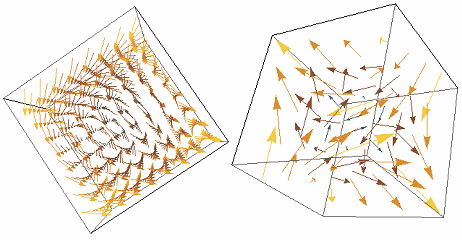
\includegraphics[scale=1.2]{./3D-vector-field.png}
  \end{figure}
  Freedom advances to a higher level when the drives ``coalesce into an
  overall viewpoint'' (134). (Note that Nietzsche objects to diversity
  on the grounds that it attenuates the unity needed for freedom.)
\end{frame}

\begin{frame}
  \frametitle{Naturalizing Freedom}
  Three candidates (135) for a more general and high-level freedom (on
  the level of organism rather than drive):
  \begin{description}
  \item[coherence] ``drives are individually strong, but also synthesized,
    organized, and unified so as to maximize the organism's overall
    success''
  \item[stable structure] ``the organism keeps a consistent view of its interests and
    runs its behaviour with a steady aim''
  \item[pyramid hierarchy] ``one ruler of the set of drives {\ldots}
    multiplicity amd disaggregation of the impulses, lack of system
    among them results in a weak will''
  \item 
  \end{description}
\end{frame}

\begin{frame}
  \frametitle{Naturalizing Freedom}
  The deliberative self in Nietzsche is often said to be either
  illusory or epiphenomenal. Richardson disagrees with this
  assessment: ``agency is indeed a kind of drive itself'' (137),
  comparable to Freud's superego. It is deluded into thinking of
  itself as Plato's charioteer, but this doesn't make it less of a
  force (and an effective cause of behaviour) in favour of herd
  instincts that cripple individuality.
\end{frame}

\begin{frame}
  \frametitle{Evolution of Agency}
  \begin{description}
  \item[Gay Science] the history of language and consciousness
    \begin{itemize}
    \item predicated on the herd, not useful for the solitary
    individual
  \item consciousness always presses towards herd mentality
  \item consciousness and language tame us into good herd animals
  \item therefore, consciousness is not epiphenomenal
    \end{itemize}
  \end{description}
\end{frame}

\begin{frame}
  \frametitle{Evolution of Agency}
  \begin{description}
  \item[Genealogy of Morals] the ability to promise
    \begin{itemize}
    \item needs memory
    \item needs inhibitive capacity (the first preschooling for
      spirituality)
    \item trains ultimately not in keeping individual, personalized
      promises; but to remember, internalize, and abide by social
      norms
    \item is deeply ascetic (140)
    \item turns drives of mastery into enforcing drives
    \end{itemize}
  \end{description}
\end{frame}

\begin{frame}
  \frametitle{Masterful Agency}
  Richardson now proceeds to describe Nietzsche's affirmation of power
  and freedom in agency (142).
  \begin{itemize}
  \item my drives are more `me' than my conscious thinking and
    choosing
  \item the masters are individuals in which this coincidence of
    drives and conscious will is achieved
  \item there is a sense in which Nietzsche is an Aristotelian here:
    masters cannot yet exist because the narrative of asceticism has
    too much of a grip on the current generation $\longrightarrow$
    virtue (in Nietzsche's case, aristocracy) can only come from an
    aristocratic habit and upbringing that breaks with asceticism
  \end{itemize}
\end{frame}

\begin{frame}
  \frametitle{Genealogy of Morals, Book II, Section 22}
  \begin{quote}
    The reader will already have conjectured what took place on the
    stage and behind the scenes of this drama. That will for
    self-torture, that inverted cruelty of the animal man, who, turned
    subjective and scared into introspection (encaged as he was in
    "the State," as part of his taming process), invented the bad
    conscience so as to hurt himself, after the natural outlet for
    this will to hurt, became blocked---in other words, this man of
    the bad conscience exploited the religious hypothesis so as to
    carry his martyrdom to the ghastliest pitch of agonized intensity.
  \end{quote}
\end{frame}

\begin{frame}
  \frametitle{Genealogy of Morals, Book II, Section 22}
  \begin{quote}
    Owing something to God: this thought becomes his instrument of
    torture. He apprehends in God the most extreme antitheses that he
    can find to his own characteristic and ineradicable animal
    instincts, he himself gives a new interpretation to these animal
    instincts as being against what he `owes' to God (as enmity,
    rebellion, and revolt against the `Lord,' the `Father,' the
    `Sire,' the `Beginning of the world'), he places himself between
    the horns of the dilemma, `God' and `Devil.'
  \end{quote}
\end{frame}

\begin{frame}
  \frametitle{Genealogy of Morals, Book II, Section 22}
  \begin{quote}
    Every negation which he is inclined to utter to himself, to the
    nature, naturalness, and reality of his being, he whips into an
    ejaculation of `yes,' uttering it as something existing, living,
    efficient, as being God, as the holiness of God, the judgment of
    God, as the hangmanship of God, as transcendence, as eternity, as
    unending torment, as hell, as infinity of punishment and guilt.
  \end{quote}
\end{frame}

\begin{frame}
  \frametitle{Genealogy of Morals, Book II, Section 22}
  \begin{quote}
    This is a kind of madness of the will in the sphere of
    psychological cruelty which is absolutely unparalleled: man's will
    to find himself guilty and blameworthy to the point of
    inexpiability, his will to think of himself as punished, without
    the punishment ever being able to balance the guilt, his will to
    infect and to poison the fundamental basis of the universe with
    the problem of punishment and guilt, in order to cut off once and
    for all any escape out of this labyrinth of `fixed ideas,' his
    will for rearing an ideal---that of the `holy God' ---face to face
    with which he can have tangible proof of his own unworthiness.
  \end{quote}
\end{frame}

\begin{frame}
  \frametitle{Genealogy of Morals, Book II, Section 22}
  \begin{quote}
    Alas for this mad melancholy beast man! What phantasies invade it,
    what paroxysms of perversity, hysterical senselessness, and mental
    bestiality break out immediately, at the very slightest check on
    its being the beast of action! All this is excessively
    interesting, but at the same time tainted with a black, gloomy,
    enervating melancholy, so that a forcible veto must be invoked
    against looking too long into these abysses.
  \end{quote}
\end{frame}

\begin{frame}
  \frametitle{Genealogy of Morals, Book II, Section 22}
  \begin{quote}
    Here is disease, undubitably, the most ghastly disease that has as
    yet played havoc among men: and he who can still hear (but man
    turns now deaf ears to such sounds), how in this night of torment
    and nonsense there has rung out the cry of love, the cry of the
    most passionate ecstasy, of redemption in love, he turns away
    gripped by an invincible horror---in man there is so much that is
    ghastly---too long has the world been a mad-house.
  \end{quote}
\end{frame}

\begin{frame}
  \frametitle{Guilt, Bad Conscience, and Self-Punishment}
  How could anything originate out of its opposite?

  \bigskip
  
  \begin{tabular}{|c|c|}\hline
    & \\
    good as in ``good and bad'' & evil \\
    & \\ \hline
    & \\
    cruelty & bad conscience \\
    & \\ \hline
  \end{tabular}
\end{frame}

\begin{frame}
  \frametitle{Guilt, Bad Conscience, and Self-Punishment}
  Two foundational type facts about humans:
  \begin{enumerate}
  \item Human beings tend to gain pleasure from inflicting suffering.
  \item When a drive is prevented from discharging itself outwardly,
    it seeks to do so inwardly.
  \end{enumerate}
  The social environment triggers the type facts to become effective.
  For Freud, repression is a similar mechanism with similar outcomes.
\end{frame}

\begin{frame}
  \frametitle{Guilt, Bad Conscience, and Self-Punishment}
  \begin{block}{psychological hedonism}
    the deepest motive of all human behaviour is the attainment of
    pleasure und the avoidance of pain (128)
  \end{block}
  \begin{block}{will to power}
    above all, a living thing wants to discharge its strength---life
    itself is will to power
  \end{block}
\end{frame}

\begin{frame}
  \frametitle{Flow Chart}
      \begin{figure}[h]
    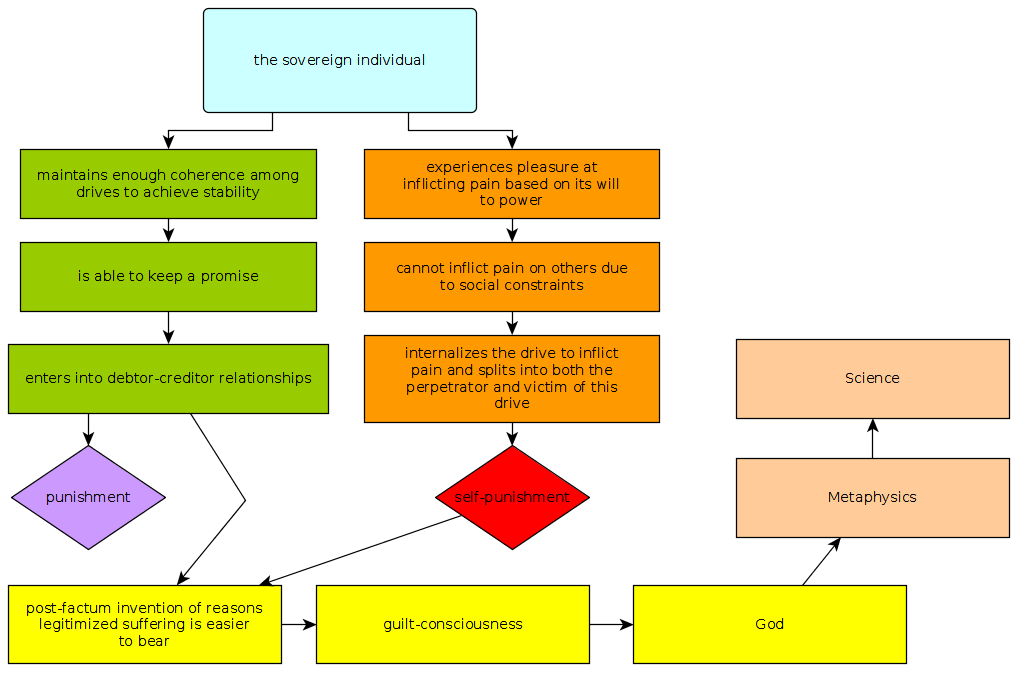
\includegraphics[scale=.35]{./janaway-nietzsche-guilt.png}
  \end{figure}
\end{frame}

\end{document}
